\chapter{TIC's en la Educación}
\label{chap:tics}

Las \Gls{tic} son un conjunto de herramientas tecnológicas y recursos utilizados
para comunicar, crear, diseminar, almacenar y manejar la
información\cite{unesco:ict}. Estas tecnologías abarcan computadoras personales,
internet, radio, televisión y telefonía\cite{tinio:ict}.

Las \Gls{tic} fueron utilizadas como complemento a la educación desde los
inicios de la misma con la radio y la televisión. Fueron vistas como un
complemento a las herramientas utilizadas en clase, como complemento del libro,
o como una herramienta que elimina la distancia física entre el profesor y el
alumno\cite{unesco:ict}. 


\section{Educación Tradicional}

La educación tradicional o instruccionismo se basa en el concepto de que existe
un profesor y un alumno. El profesor transfiere el conocimiento que ha adquirido
de diferentes métodos (educación, experiencia, etc) a un alumno que es un
receptor pasivo de información\cite{johnson2005instructionism}.

Se enfoca más en el profesor, en la capacidad del mismo, y en el producto final
como resultado de un proceso no interactivo y bien
documentado\cite{igi:instructionism}. Los mecanismos tradicionales para poder
probar la efectividad de este tipo de enseñanza son los exámenes.

La principal critica a este modelo es que se enfoca la enseñanza y no el
aprendizaje, mientras más se enseña, más se aprende. Esto contradice al sentido
común en el sentido de que, cosas básicas como caminar o hablar, aprendemos sin
la necesidad de un
profesor\cite{ackoff:education}\cite{johnson2005instructionism}.

Tradicionalmente el rol de las TIC's en la educación se vio relegada a la de
sustituto del libro y/o de presentaciones en clase, es decir, es un mecanismo
más para trasmitir el conocimiento del maestro al alumno.



\section{Educación con TIC's}
\label{sec:tics_EDUCACION_TICS}

Las expectativas iniciales acerca del impacto de las \Gls{tic} en la educación
fueron ampliamente superiores a los resultados obtenidos\cite{unesco:ict}, con
el advenimiento de las computadoras esta brecha se redujo, en mayor medida por
que se las utilizo en conjunto con tecnologías como Internet, y los efectos
positivos en la educación fueron aumentando gradualmente\cite{unesco:ict}.

Las principales ventajas de la utilización de las \Gls{tic} en la educación es
su aplicabilidad en áreas que no pueden ser cubiertas por otras alternativas,
como son:

\begin{description}

    \item[Nuevos modelos pedagógicos] teorías como el constructivismo moderno
	    enfatizan el proceso de como adquirir conocimiento y no solamente el
	    conocimiento en sí.

    \item[Eliminación de distancias] Con el advenimiento de las computadoras y los
	    satélites, el mundo se ha convertido en una aldea global, y las
	    distancias en cuestiones de transmisión de información se han vuelto
	    insignificantes\cite{mohammed2013information}, los medios
	    tradicionales como bibliotecas, o escuelas están limitados a un
	    espacio físico, con el uso de las \Gls{tic}, esta restricción
	    física desaparece\cite{tinio:ict}.

    \item[Colaboración distribuida] como consecuencia del punto anterior, los
	    alumnos pueden colaborar de manera más sencilla pues no tienen
	    limitaciones físicas. Además, los alumnos pueden consultar con
	    expertos que están en linea, e incluso tener mentores en linea,
	    estas tutorías pueden ser uno a uno, por ejemplo mediante
	    comunicaciones por correo electrónico. Además permite la
	    colaboración masiva entre estudiantes de intereses comunes, mediante
	    foros y redes sociales\cite{unesco:ict}.

    \item[Motivación para aprender] Las \Gls{tic} tienen un impacto positivo en
	    el proceso de aprendizaje especialmente en lo referente al
	    compromiso con la actividad (a través de estímulos visuales,
	    auditivos, etc), capacidad de investigación (es más fácil acceder a
	    gran cantidad de información bibliográfica), capacidad de escritura
	    y lectura (permitiendo compartir ideas de manera más legible y
	    mejorarlas iterativamente) y capacidad de presentación (es más fácil
	    presentar trabajos profesionalmente a un público
	    mayor)\cite{passey2004motivational}\cite{egenfeldt2007third}.

    \item[Adquisición de habilidades básicas] las habilidades necesarias para
	    utilizar de manera efectiva las \Gls{tic} se están convirtiendo en
	    una necesidad básica, un aprendizaje guiado por las mismas puede
	    ayudar a una rápida asimilación de los conceptos relacionados.

\end{description}

Uno de los desafíos más importantes que enfrentan las \Gls{tic} para convertirse
en una alternativa viable es la inversión en infraestructura
necesaria\cite{unesco:ict}. 

\subsection{Historia}

La historia de las \Gls{tic} en educación comienza con la Universidad Abierta
del Reino Unido\footnote{Open University of United Kingdom} que en 1969 se
establece como la primera institución educativa dedicada a la enseñanza a
distancia utilizando las, para aquel entonces, nuevas
tecnologías\cite{tinio:ict}.

En 1973 Vint Cerf creo el protocolo TCP/IP y es considerado el nacimiento de
Internet\cite{white:ict}, lo que permitió que la información pueda ser
transmitida de manera más sencilla, tiempo después con la aparición de las
computadoras personales en 1977\cite{white:ict}. 

Otro hito tecnológico se dio en la \Gls{cern} en el año 1989 cuando se concibió
lo que hoy se conoce como \emph{World Wide Web}, permitiendo que los usuarios de
la \emph{Web} puedan compartir archivos mediante un protocolo
estándar\cite{white:ict}. 

Con las principales eventos que marcaron la evolución tecnológica de las
\Gls{tic} en la educación, se divide su historia en cinco partes. Las mismas se
pueden dividir en dos secciones, las primeras tres corresponden a los comienzos
y donde los alumnos eran receptores de información, época denominada
\emph{pull}, y la segunda denominada\emph{push}\cite{white:ict} que es aquella
donde los alumnos participan de su educación y son creadores activos de
conocimiento.

\subsubsection{Programación, ejercicios y prácticas}

Este periodo que abarca desde la aparición de las primeras computadoras
personales hasta el final de la década de 1980, este periodo se caracterizo por
computadoras muy limitadas, ausencia de interacción multimedia y escasez de
programas especializados. Se enseñaba programación básica\cite{leinonen:ict}, no
por la necesidad de educar programadores, sino por la creencia de que así se
desarrollarían habilidades matemáticas y lógicas en los alumnos. 


\subsubsection{Edutainment}
\todox{Debería ser un nivel más anidado.}

En este periodo se desarrollaron una gran cantidad de aplicaciones educativas
que más tarde serían conocidas como \emph{Edutainment}\footnote{Education +
	Enteirtainment, se traduce como educación entretenida}, estas pretendían
agregarle entretenimiento a la educación, se veía al como un receptor pasivo de
información que debía asimilarla, y para aumentar el compromiso, el
entretenimiento era agregado\cite{resnick:2004}.

Esta basado principalmente en la teoría del conductismo y el cognoscitivismo, se
enfoca en juegos sencillos que transmiten información simple al usuario, siendo
este un receptor pasivo de información, su estructura se basa en un objetivo
claro que esta separado de la experiencia educativa\cite{egenfeldt2007third}.
Math Blaster (ver~\ref{fig:math_blaster}) es un \emph{edutainment} donde el
alumno debe responder repetitivamente preguntas aritmeticas para obtener
municiones, luego con esas municiones debe completar diferentes misiones en una
nave\cite{bruckman1999can}. Como todas las preguntas se responden mediante un
mecanismo de selección múltiple, y no existe penalización por fallar una
respuesta, rapidamente los alumnos seleccionan cualquier opción, si no es la
correcta, eligen la siguiente, y repiten el proceso hasta obtener la respuesta
correcta, este proceso es conocido como \emph{prueba y error sistemático}. 

\begin{figure}[h!] 
	\centering 
	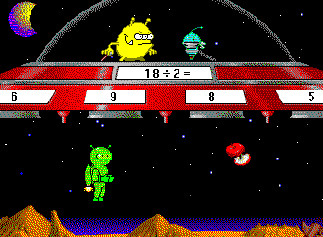
\includegraphics[scale=0.5,natwidth=296,natheight=217]{tics/math_blaster.jpg}
	\caption{Math Blaster, \emph{edutainment} del año 1987}
	\label{fig:math_blaster} 
\end{figure}

Los \emph{edutainment} fallaron en enseñar habilidades no triviales, se enfocan
principalmente enseñar tareas extremadamente repetitivas que no dependen de un
contexto\cite{charsky:2010}\cite{egenfeldt2007third}\cite{bruckman1999can}, son
excelentes para enseñar a sumar, pero no para aplicar ese conocimiento, analizar
y obtener conclusiones, o evaluar lo que aprendieron.

Las principales causas por las cuales los \emph{edutainment} fracasaron en su
intento de ser una alternativa viable a la educación son según
\cite{egenfeldt2007third}: 

\begin{description}

    \item[Falta de motivación interna] la única forma que tenían de intentar que
	    el alumno quiera seguir jugando eran las recompenzas, que eran muy
	    seguidas y fáciles de conseguir.

    \item[Aprendizaje como anexo] el principal objetivo del desarrollo de los
	    \emph{edutainment} eran el de entretener, los objetivos pedagógicos
	    eran agregados al final. Se enviaban informaciones al alumno
	    mediante largos textos que normalmente eran omitidos.
    
    \item[Jugabilidad sencilla] la mayoría eran sencillos juegos de arcade, la
	    mayor parte de la interacción eran a traves de palabras que eran
	    presentadas en forma de selección multiple. 

    \item[Ejercicios de prueba y error sistemáticos] todas las debilidades
	    anteriores se pueden fundamentar en el hecho de que los juegos
	    permitían al alumno intentar varías veces antes de dar una opción
	    correcta, sumando esto al echo de que los mismos no estaban
	    motivados, provocaba que todas las opciones sean probadas sin el
	    proceso de reflexión necesario para aprender, por ejemplo, varios
	    juegos aritméticos solicitaban pruebas del tipo
	    \begin{math}{2+2}\end{math} el alumno probaba diferentes resultados
	    y luego memorizaba el mismo. Se enseñaba a probar opciones sin
	    sentido antes que entender y analizar la experiencia.

\end{description}

\subsubsection{Entrenamiento basado en computadoras}

Cuando aparecieron en el mercado computadoras con multimedia, se argumento que
los ejercicios de la era anterior fallaron en su objetivo de una educación
profunda por que no contenían multimedia\cite{leinonen:ict}, las aplicaciones
eran distribuidas por CD-ROM, y así se actualizaban de manera más frecuente, y
podían contener gran cantidad de contenido multimedia.

Las bases pedagógicas de esta se basada en la capacidad de ciertos estudiantes
de aprender mejor cuando interactúan con contenido multimedia, la \emph{prueba y
	error} aún estaban presentes, pero no eran presentados inmediatamente,
sino más bien una vez que el alumno ya debería haber asimilado los conceptos y
funcionaban como pruebas de adquisición de conocimiento. Este tipo de contenido
tampoco logro la enseñanza profunda, solamente fueron efectivos en el
aprendizaje de idiomas, fallando en todos los demás campos\cite{leinonen:ict},
además los contenidos muchas veces estaban desactualizados y obtener nuevas
versiones no era una tarea sencilla.

Varios gobiernos apoyaron de manera agresiva la introducción de las \Gls{tic} en
educación\cite{mcdougall2006theory} y se realizo un importante avance teórico
con los trabajos sobre el aprendizaje construccionista de Papert y Harel (1991),
y la influencia de las computadoras sobre el aprendizaje y la mente de Marvin
Minksy (1987)~\cite{mcdougall2006theory}.

A comienzos de la decada de 1990, con la popularización de Internet, se le vio
como solución al problema de las poco frecuentes actualizaciones de aplicaciones
educativas, su utilización no tenia bases pedagógicas, más bien se basaban en la
facilidad de distribuir contenido por la \emph{Web}, el principal inconveniente
era la velocidad del Internet, no era suficiente para proveer entornos ricos en
multimedia como lo hacían los CD-ROM\cite{leinonen:ict}.

\begin{figure}[ht!] 
	\centering 
	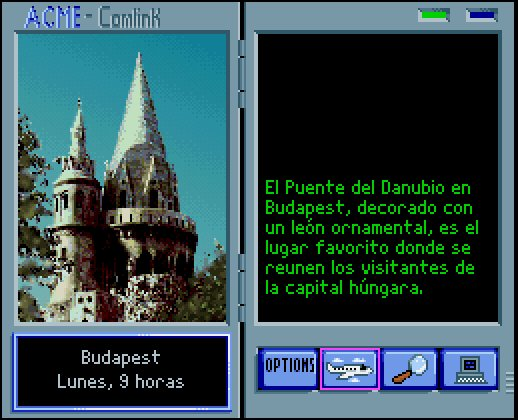
\includegraphics[scale=0.5]{tics/carmen.jpg}
	\caption{Donde en el mundo esta Carmen Sandiego} 
	\label{fig:carmen}
\end{figure}

Donde en el mundo esta Carmen Sandiego (ver~\ref{fig:carmen}) es un juego que
representa el potencial multimedia de esta época, el objetivo del juego era
detener a una serie de criminales mediante una serie de pistas que eran
provistas en forma de texto\cite{charsky:2010}. Este exitoso juego demuestra las
falencias de esta época, siendo visualmente muy atractivo, y con contenido
multimedia acorde a su tiempo, no era más que prueba y error, cada nivel del
juego podía ser completado sin leer el texto que contenía la información
educativa.

Todos los errores cometidos en la época anterior estaban presentes nuevamente,
no se establecieron marcos teóricos que fundamentasen la utilización de
contenido multimedia, así, se solucionaron los problemas de simplicidad, pero se
demostró que el principal problema era la prueba y error sistemático y sin
sentido\cite{egenfeldt2007third} 

\subsubsection{e-Learning}

La bases pedagógicas de esta son similares a la era del entrenamiento basado en
computadoras, se distribuye contenido masivamente a los alumnos, y luego, de
manera muy discreta se permite a los mismos colaborar, dejando siempre en claro
que primero se debe asimilar toda la información posible y luego relacionarse
con los demás\cite{leinonen:ict}.

\emph{E-Learning} se define como la educación y capacitación a traves de medios
digitales, incluye todo tipo de media capaz de distribuir información, puede ser
síncrono o asíncrono, y es particularmente útil para educación a distancia y con
horarios flexibles. Se origino a finales de la década de 1990 y tubo su apogeo a
mediados de la década del 2000, apoyada por la gran penetración de las \Gls{tic}
en la población\cite{punie:ict}.

Todos los paradigmas anteriores viven dentro del \emph{e-Learning}, permitiendo
compartir contenido multimedia y realizar pruebas del tipo \emph{prueba-error}. 

\begin{figure}[h] \centering 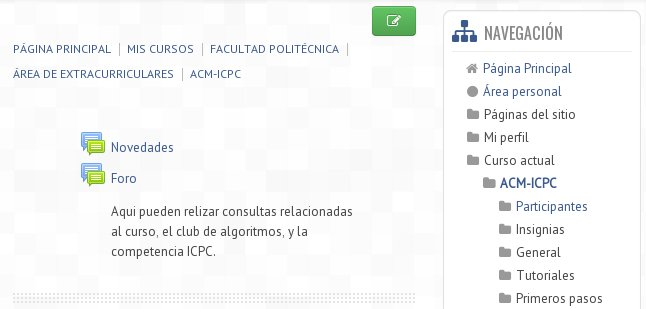
\includegraphics[scale=0.5]{tics/moodle.jpg}
	\caption{Moodle, plataforma de e Learning} \label{fig:moodle}
\end{figure}

La plataforma \emph{Moodle} (ver~\ref{fig:moodle}) cuya primera versión salio en
el 2002, es una de las principales herramientas del \emph{e-Learning} hoy en
día, permite la creación de cursos específicos por materia y sitios
especializados por instituciones académicas\cite{perkins2006using}. 

Si bien en las anteriores épocas, el uso de las \Gls{tic} estaba más orientado
hacia la educación básica y secundaría, el \emph{e-Learning} actualmente es más
utilizado en la educación terciaría\cite{punie:ict}.

La utilización del \emph{e-Learning} tiene varios grados de aplicación en
entornos reales\cite{punie:ict}, que van desde ser simples elementos
complementarios a la clase, como por ejemplo un repositorio para las
diapositivas y otros materiales de clase, hasta cursos completamente en linea,
donde la clase ha sido completamente sustituída.

\section{Problemas actuales}

Durante la historia de las \Gls{tic} en la educación, se han encontrado
diferentes dificultades a la hora de aplicar los nuevos conceptos en la
educación, desde los primeros enfoques que carecían de bases pedagógicas válidas
hasta la actualidad, el principal problema es falta de motivación de los
profesionales de la educación para emplear las
\Gls{tic}\cite{punie:ict,ict:romeo}.

\todox{Reconsiderar el párrafo que esta comentado bajo este todo}
%\fixme{El contenido proveído actualmente puede ser considerado como un conjunto
%    de buenas prácticas\cite{punie:ict} y así, omiten completa o parcialmente el
%    contexto donde esa buena práctica fue generado. }{No se entiende de donde
%    sale esto, de que habla y para qué?}

Aún así, las \Gls{tic} han tenido un impacto positivo en la educación, pero el
mismo no es el esperado\cite{punie:ict}, por ejemplo, iniciativas como el
\emph{edutainment} que prometían ser la solución a los problemas
educacionales no cumplieron las expectativas. 

Sucesivos fracasos en los resultados obtenidos dotaron a los \emph{edutainment}
de una reputación negativa, y hoy en día son considerados como un método educativo 
ineficiente, pues son un ejercicio de \emph{prueba-error}
ocultos bajo un juego poco entretenido\cite{resnick:2004}, además de su
incapacidad de enseñar como aplicar conceptos aprendidos a un entorno
real\cite{resnick:2004}.


Mientras que la utilización de las \Gls{tic} puede eliminar problemas actuales
como el aislamiento y la falta de pensamiento de alto nivel\cite{punie:ict}, la
brecha social existente implica otro riesgo para la utilización de las \Gls{tic}
en la educación, aquellos que no posean los recursos económicos necesarios para
acceder a la misma no se verán beneficiados por las \Gls{tic}\cite{punie:ict}.

\fixme{Empresas que están en el área de las \Gls{tic}}{Mejorar/pulir lengua} en
educación siguen en la época donde los juegos son prueba y error, esto no
significa que los mismos no funcionen, sino que pueden ser mejorados
considerablemente\cite{egenfeldt2007third}.

Otro de los desafíos actuales es la dificultad comercial impuesta por la
historia de los mismos, es muy difícil para los juegos actuales presentar
promesas realistas, principalmente por el antecedente sentado por los
\emph{edutainment}\cite{egenfeldt2007third}

\section{Construccionismo y las TIC's}
\label{sec:tics_CONSTRUCCIONISMO}

\fixme{El construccionismo es una corriente}{decir primero que es, antes de
    comprara} pedagógica con un enfoque diferente en cuanto al uso de las
\Gls{tic} en la educación. Esta pedagogía se diferencia de la educación
tradicional en que el estudiante ya no es un receptor pasivo de información, en
cambio, el mismo participa activamente del proceso de aprendizaje construyendo
su propio conocimiento. 

\fixme{El construccionismo}{no repetir} utiliza la tecnología como medio
cognitivo  a \fixme{diferencia}{} de la educación tradicional que la utiliza para la
entrega de contenido. 

\fixme{El construccionismo}{no repetir} es un alternativa prometedora a la
educación tradicional. Desde el punto de vista tecnológico, el construccionismo
es ideal pues el mismo requiere un alto dinamismo en el traspaso del
conocimiento \cite{sasha:construtivism}. 

\fixme{El construccionismo}{no repetir} y las \Gls{tic} siempre han estado
relacionados, ya que el mismo se originó con un lenguaje de programación
(LOGO)\cite{ict:ttc}. Un característica importante de esta relación es que
tienen la capacidad de eliminar los problemas de
distancia\cite{mariluz:seiousgames}.


\subsection{Historia}

En la decada de $1980$, \emph{Seymour Papert} adoptó el término construccionismo
para representar una método pedagógico practicado por \fixme{John Dewey}{?} a
principios del siglo 20. Este método buscaba que la responsabilidad de aprender
recaiga en el estudiante. 

Papert trabajó directamente con el psicólogo evolutivo y filósofo suizo Jean
Piaget. \fixme{Este}{qué?} último, había elaborado con anterioridad sus teorías
de la educación y construcción del conocimiento al ver e interactuar con los
niños y a partir de esta observación dio origen al constructivismo, según el
cual, el conocimiento debe ser construido por el estudiante y los nuevos
significados deben ser obtenidos relacionándolos con significados anteriores por
los mismos estudiantes haciendo uso así de sus propios sistemas de relaciones.

El construccionismo se \fixme{diferencia}{} de lo anterior en que los estudiantes
construyen las ideas o partes del mundo utilizando herramientas. La elaboración
de representaciones mentales mediante la construcción y el intercambio es la
metáfora del marco construccionista. 

Durante $1980$, Seymor Papert, Wally Feurzeig, Marvin Minsky y John McCarthy y los
miembros del Departamento de Inteligencia Artificial del \Gls{mit} y una
compañía de tecnología en Cambridge, Massachusetts, desarrollaron un nuevo
lenguaje de programación llamado LOGO que tenía por objeto que los estudiantes
construyeran sus \fixme{modelos}{que modelos} en notación LOGO@. Este juego
introduciría de forma natural las ideas de los procedimientos, funciones,
variables, recursividad, la modularidad, simulación, verificación, entre otros.

La creación del lenguaje de programación LOGO dio inicio al construccionismo.

Los desarrolladores de LOGO no solo alentaron la promoción de formas
construccionistas de enseñanza y aprendizaje sino también alentaron otra forma
de aprendizaje nueva y no tradicional con las diferentes herramientas tecnológicas. 

De vuelta en la década de 1980, cuando se produjo LOGO y se acuñó el
construccionismo, la comunidad del construccionismo era en su mayoría  ingenieros
informáticos y matemáticos\cite{historia:2014}.

\observacion{Toda la sección hay que reordernar}

\subsection{Bases Pedagógicas}

Para el construccionismo, el conocimiento es construido por el estudiante en
lugar de ser trasmitido por el \fixme{profesor}{explicar el rol del profesor en
    el construccionismo}\cite{moses:2003} y esto sucede particularmente cuando
el mismo se compromete en la elaboración de un producto o artefacto que tenga un
significado y pueda ser compartido\cite{valdivia:sg}. De esta manera, se permite
a los estudiantes elaborar sus propias interpretaciones razonadas del mundo
mediante la interacción con el mismo.

Según Papert, los alumnos estarán mucho más involucrados en su aprendizaje si
construyen artefactos que los demás pueden ver, criticar y tal vez utilizar. Y
además, el alumno se enfrenta a problemas complejos con estas construcciones,
harán el esfuerzo por resolver problemas y aprender ya que la construcción les
motivará\cite{const:vs}.

El enfoque construccionista establece que los seres humanos conocen y aprenden
de formas diferentes por lo tanto, no se puede elaborar una jerarquía de estilos
de aprendizajes\cite{valdivia:sg}.

\subsection{\fixme{Estado del Arte}{Construccionismo en la presente}}

El construccionismo pone énfasis en el \emph{Aprender haciendo}, esta idea
\fixme{mejora}{ref} la práctica educativa tradicional o instruccionismo. El instruccionismo
se basa en el concepto de que existe un profesor y un estudiante, el profesor
transfiere el conocimiento que ha adquirido a un alumno que es receptor pasivo
de información de esta manera, se enfoca más en la capacidad del profesor. 

Existen varios emprendimientos o \emph{\fixme{amigos del contruccionismo}{?}},
para la mayoría de ellos las computadoras son esenciales mientras que para otros
el mayor esfuerzo está en la incorporación de la tecnología en su práctica
educativa\cite{papertian:const}.

Algunos de estos emprendimientos son:

\observacion{Cambiar el ``description'' por ``itemize''}
\begin{description}

\item[Lenguaje de programación LOGO]  A mediados de la década de 1960 Seymour
	Papert, que había estado trabajando con Piaget en Ginebra, llegó a
	Estados Unidos donde co-fundó el Laboratorio de Inteligencia Artifical
	del MIT con Marvin Minsky. Papert trabajó con el equipo de Bolt, Beranek
	y Newman, liderado por Wallace Feurzeig, que creó la primera versión del
	logotipo en 1967. A lo largo de la década de 1970 Logo fuen incubado en
	el MIT y algunos otros sitios de investigación. El lenguaje de
	programación Logo, un dialecto de Lisp, fue diseñado como una
	herramienta para el aprendizaje. Sus características como la
	modularidad, extensibilidad, interactividad y flexibilidad se derivan de
	este objetivo. 
	%http://el.media.mit.edu/logo-foundation/logo/index.html

	El lenguaje Logo es la cuna del construccionismo, se basa en el
	principio de que se aprende mejor haciendo, pero se aprende todavía
	mejor si se combina la acción con la verbalización  y la reflexión
	acerca de lo que se ha hecho. Fundamentalmente consiste en presentar a
	los niños retos intelectuales que puedan ser resueltos mediante el
	desarrollo de programas en Logo. El proceso de revisión manual de los
	errores contribuye a que el niño desarrolle habilidades metacognitivas
	al poner en práctica procesos de auto-corrección\cite{logo:sg}.
	%http://es.wikipedia.org/wiki/Logo_(lenguaje_de_programaci%C3%B3n)

    \observacion{Ver que decir  qu eno sea repetitivo con todo lo que ya se
        dijo.}


%\item[Simulación] La simulación en el ámbito de la educación fue evolucionando
%desde simples motores de reglas hasta complejos entornos, la simulación
%demostró ser una herramienta muy útil el ámbito laboral
%\cite{mariluz:seiousgames}, pues enseña al alumno a encarar situaciones muy
%difíciles de representar en entornos completamente controlados y provee
%mecanismos para comprobar la efectividad de la herramienta. 

%Actualmente la simulación se utiliza más en el ámbito empresarial pues las
%empresas son las más necesitas de innovar en el ámbito de la enseñanza. Un
%ejemplo de esta necesidad se da, por ejemplo, en el entrenamiento de nuevos
%vendedores, es muy difícil enseñar a un vendedor como debe vender los productos
%con un pizzarón y/o una presentación, en cambio la simulación permite que el
%mismo pueda probar cosas nuevas y experiencias de sus compañeros (o
%instructor), convirtiendo así el aprendizaje en
%colectivo\cite{mariluz:seiousgames}. En el ámbito académico la simulación mas
%utilizada en campos físicos (como simulación de fluidos), meteorología
%(simulación de tormentas y fenómenos climáticos), etc. 

%\item[Serious Games] Diseñado con el propósito de aprender. Generalmente hace
%uso de la simulación para permitir un aprendizaje más realista.

%\item[Lego Serious Play] Es una iniciativa de Lego que busca fomentar el
%pensamiento creativo por medio de la construcción por parte de los estudiantes
%de su identidad y experiencias utilizando legos. 

\item[\Gls{olpc}]. El esfuerzo se centra en dotar a los niños de una computadora
	duradera, accesible y potente en los países en desarrollo, se dice que
	es un descendiente directo del construccionismo. Con esto se busca que
	la computadora personal sea utilizada como un laboratorio intelectual y
	un vehículo para la auto-expresión. OLPC no tiene que ver con la
	escolarización o la escuela, más bien las utiliza como medio de
	distribución de las computadoras a los niños, los cuales pueden
	utilizarlas para aprender en cualquier lugar y momento. Se busca
	fomentar el aprendizaje natural, es decir, aquel aprendizaje sin
	enseñanza.

    \fixme{Los problemas atribuidos al experimento}{experimento?} OLPC son
    predominantemente las críticas a la política, el liderazgo o de la
    intransigencia de la escuela en vez del construccionismo o computadora
    personal para los niños pobres. El experimento audaz de Nicholas Negroponte
    (co-fundador de \Gls{olpc}) y Sugata Mitra para dejar las computadoras desde
    un helicóptero sobre una aldea de África se basa en la creencia en el
    construccionismo\cite{papertian:const}.

    \observacion{Poner referencias}
    \observacion{Terrible descripción del proyecto OLPG}
    \observacion{No se de que portal sacaron esta descripción}

\item[Fabricación personal] Neil Gershenfeld, colega de Papert en el Media Lab
	del \Gls{mit} dictó un curso titulado \emph{Cómo hacer casi cualquier
		cosa}. La idea se centraba en la creación de  la tecnología que
	se necesita para resolver los problemas que se poseen. Esta
	auto-confianza, la autonomía personal y la agencia sobre la tecnología
	han estado en el centro de trabajo de Papert durante años. Papert no
	sólo defendió la idea de que los niños posean computadoras personales,
	sino también que a la larga ellos debían mantenerlas, repararlas e
	incluso construirlas.

	Junto con la capacidad para utilizar la tecnología para inventar
	soluciones a los problemas de significado personal, los estudiantes no
	sólo tienen acceso a la información, sino que tienen una mayor capacidad
	para darle forma a su mundo. La fabricación personal promueve la visión
	de Papert \emph{Si se puede utilizar la tecnología para hacer las cosas,
		usted puede hacer las cosas muchos más interesantes y usted
		puede aprender mucho más haciéndolo}\cite{papertian:const}.

\end{description}

%http://constructingmodernknowledge.com/cmk08/wp-content/uploads/2012/10/StagerConstructionism2012.pdf


\section{Simulación}
\label{sec:tics_SIMULACION}

\obervacion{No se entiende como se llego a esto}

\observacion{Ver como organizar el contenido para que no sea una bolsa de
    conceptos}.

La simulación se define como el proceso de diseñar un modelo de un sistema real
y, llevar a cabo experimentos con este modelo, con el fin o bien de entender el
comportamiento del sistema o de la evaluación de distintas estrategias para la
operación del sistema\cite{ingalls2008introduction}. 
%[ingalls2008introduction]

Un juego y una simulación podrían llegar a ser muy parecidos, a veces los juegos
tienen motores de simulación\footnote{Un motor de simulación es un conjunto de
objetos y métodos que se utilizan para la construcción de modelos de
simulación que están dentro de las aplicaciones}, una de las diferencias
es que la simulación es muy dependiente del contexto. 

La simulación en el ámbito de la educación fue evolucionando desde simples
motores de reglas hasta complejos entornos, la simulación demostró ser una
herramienta muy útil en el ámbito laboral\cite{mariluz:seiousgames}, pues enseña
al alumno a encarar situaciones muy difíciles de representar en entornos
completamente controlados y provee mecanismos para comprobar la efectividad de
la herramienta. 

Actualmente la simulación se utiliza más en el ámbito empresarial pues las
empresas son las más necesitadas de innovar en el ámbito de la enseñanza. Un
ejemplo de esta necesidad se da, por ejemplo, en el entrenamiento de nuevos
vendedores, es muy difícil enseñar a un vendedor como debe vender los productos
con un pizarrón y/o una presentación, en cambio la simulación permite que el
mismo pueda probar cosas nuevas y experiencias de sus compañeros (o instructor),
convirtiendo así el aprendizaje en colectivo\cite{mariluz:seiousgames}. En el
ámbito académico la simulación es más utilizada en campos físicos (como simulación
de fluidos), meteorología (simulación de tormentas y fenómenos climáticos), etc. 

Existen dos tipos de simulaciones, en primer lugar están las experimentales que
ponen al estudiante en el lugar de un profesional y requieren que el mismo tome
decisiones para alcanzar los objetivos y en segundo lugar están las simbólicas
que buscan que el estudiante deduzca eventos, principios y mejores prácticas
\cite{charsky:2010}. 

\fixme{Una simulación}{sección?} esta conformada por:

\begin{description}

\item[Entidades] Cualquier objeto o componente en el sistema que requiera
	representación explícita en el modelo se define como
	entidad\cite{banks2000dm}. Las entidades poseen atributos. Los atributos
	son las características de una determinada entidad que son exclusivos de
	esa entidad. Por último, son aquellas que cambian el estado de una
	simulación. Ejemplo de entidades son: un médico o una jeringa en una
	simulación médica.

\item[Acciones] Las entidades interactúan entre sí a través de acciones. Estas
	acciones puede causar cambios en el estado de la simulación además de
	eventos. Ejemplo de una acción en una simulación médica es la
	esterilización de un instrumento.

\item[Eventos] Los eventos son hechos que ocurren de manera controlada pero no
	siempre predecible en el entorno simulado, los mismos afectan a las
	entidades y deben obligar a realizar alguna de las acciones disponibles
	para tal evento. Ejemplo de un evento en un simulación médica es un paro
	cardíaco del paciente.

\end{description}

La confianza en el modelo o la simulación según\cite{DoDSysEng2001} se establece
mediante:

\begin{description}

\item[La verificación] Es el proceso de determinar si la implementación
	representa con precisión las especificaciones del diseño. 

\item[La validación] Es el proceso de determinar el grado en el que el modelo
	representa de forma exacta la realidad de acuerdo al uso que se tiene
	previsto darle y el nivel de confianza que debe tenerse en la
	evaluación.

\item[La acreditación] Es el proceso de certificación de un modelo para su uso
	con un propósito específico.
%[DoDSysEng2001]

\end{description}



%En la actualidad, la utilización de la simulación como herramienta para el
%entrenamiento es cada vez mayor por partes de los profesores, quienes están
%cada vez más familiarizados con la tecnología. 

%Según\cite{humphreys2013developing} los tipos de estudiantes definidos por Kolb
%son:

%\begin{description}

%\item[Accommodating learners] Aprenden de la experiencia e interiorizan el
%aprendizaje a través de experimentación activa. 

%\item[Diverging learners] Aprenden a través de experimentación activa, e
%interiorizan el conocimiento reflexionando sobre la experiencia. 

%\item[Coverning learners] Aprenden a través del pensamiento abstracto e
%interiorizan el conocimiento a través de la experimentación activa.

%\item[Assimilating learners] Aprenden a través del pensamiento abstracto y las
%interiorizan reflexionando sobre las mismas. 
	
%\end{description}

%Teniendo en cuenta el caso de la enfermería, la misma es una ciencia que atrae
%a alumnos del tipo \emph{Diverging learners}, y la simulación es una
%herramienta ideal para este tipo de estudiantes.

La mayoría de la literatura encontrada acerca de la simulación y los cuidados de
la salud no proporcionan muchos detalles acerca de la implementación de modelos
de simulación en áreas amplias, se cree que esto se debe a la complejidad de
representar las actividades relacionas al cuidado de la salud dentro de un
modelo de simulación que debe, de hecho, ser una simplificación de las mismas.
Esta simplificación puede ser un proceso sumamente complejo, por lo cual la
mayoría se centra en una parte de las actividades hospitalarias pero no así en
todas. Cuanto mayor sea el detalle, la simulación \fixme{conducirá}{} a una representación
más realista lo cual aumenta la confianza en los grupos de interés, sin embargo,
más detalle requiere más datos validados y esto puede ser costoso de
obtener\cite{guna:simulation}.

Algunas aplicaciones específicas en el cuidado de la salud son:
\observacion{Incluir un párrafo porque el énfasis en simulación y salud}

\begin{description}

\item[Departamento de emergencia y accidentes] La mayoría de los trabajos
	realizados en esta área se refieren a la optimización de tiempo de
	espera de los pacientes y la organización del personal, de las
	habitaciones,de las ambulancias, para dar mejor atención a los
    pacientes. Un ejemplo de esto es \emph{Edsim} que se utiliza para aumentar
    el rendimiento en un departamento de emergencias en los Estados Unidos como
    parte de un sistema que permite el desvío de ambulancias en los períodos
    pico de demanda, el cual incluye la introducción de salones de descarga y la
    disminución del tiempo de estancia, sin pasar por el
    triaje\cite{guna:simulation}. 
	
\item[Instalaciones para pacientes hospitalizados] Los trabajos se centran en la
    mejora en la atención con respecto al flujo de pacientes así como la
    ocupación de camas. Muchos trabajos tratan de demostrar como se podrían
    utilizar modelos matemáticos para esto. \emph{Harper y Shahani} presentaron
    un modelo de simulación flexible relacionado a estás cuestiones de pacientes
    hospitalizados, el mismo utiliza \emph{TOCHSIM}, \fixme{flexible en el sentido de
        que aborda también}{pulir} problemas como la creación de una nueva
    unidad en el hospital\cite{guna:simulation}.

\item[Clínicas para pacientes ambulatorios] \fixme{En este sentido}{?} la
    simulación se utiliza para minimizar el tiempo de espera de los pacientes en
    clínicas externas, \fixme{es decir}{pulir}, aquellas en las que se sacan citas. El tiempo
    de espera no sólo implica la espera dentro de la clínica sino también el
    tiempo que pasa entre el momento en el que se solicita un cita y el día de
    la cita. Un ejemplo de esto es \emph{CLINSIM} que se utilizó en el Reino
    Unido para observar como la política de operación puede influir en los
    tiempos de espera de los pacientes\cite{guna:simulation}. 

\item[Formación médica y quirúrgica] Se centran en tareas específicas y en la
	formación de un conjunto limitado de habilidades referentes a estas
	tareas. Los ejemplos más recientes son entrenamiento para un intubación
	esofágica, capacitación y evaluación de capacidades laparoscópicas,
	entrenamiento para la palpación de tumores de mama\cite{mantovani:vr}. 

\item[Sistemas de formación de emergencias] Se refieren a aquellas simulaciones
	diseñadas para la rápida respuesta médica. Incluye desde pacientes
	virtuales dinámicos cuya acción por parte del estudiante produce un
	cambio clínico en el mismo y una respuesta al estudiante.  Otro ejemplo
	es el utilizado en la marina de EE.UU que intenta formar a los
	profesionales para su rápida acción frente a desastres civiles y donde
	la estabilización de pacientes se tenga que dar con recursos
	limitados~\cite{mantovani:vr}. 

\item[Entrenamiento para profesionales de salud mental] Janssen LP creó una
	simulación para educar a los psiquiatras y profesionales de la salud en
	lo que es tener esquizofrenia llamada \emph{el viaje en autobús} que
	trata de mostrar lo que pasa dentro de de la mente de una persona con
	esquizofrenia cuando viaja en autobús en base a experiencias relatadas
	por pacientes y médicos\cite{mantovani:vr}. 

\end{description}

\observacion{Buscar manera de poner todas estas secciones en un mismo plano,
    como para que tenga sentido el ir explicándolas (falta un conector), por
    ejemplo, donde se sitúan todos estos trabajos en la linea de tiempo que
    presentaron inicialmente? Esta demasiado desconectado e aislado.
    
    Se necesita complementar mas esa primera sección de manera tal a que se
    entienda de donde salio todo esto.}

\section{Gamification}
\label{sec:tics_GAMIFICATION}
\todox{Agregar mas contenido}

Es el uso de mecánicas tradicionalmente usadas en los videojuegos en contextos distintos
a los juegos. Según Shell \cite{hj:gamification} un juego es una actividad cuyo fin es resolver un problema de manera entretenida. 

La \emph{Gamification}, mejora la actividad del usuario, el \emph{engagement} (enganchamiento o compromiso con el juego), el aprendizaje, la puntualidad (capacidad de completar una tarea o asignación antes del tiempo designado), el retorno a la inversión, la calidad y la colaboración.

\subsection{Principios}

Los principios de la gamification moderna según \cite{hj:gamification} son los 
siguientes:

\begin{itemize}
\item Objetivos bien definidos.
\item Mejor registro de resultados y tablas de puntuación.
\item Retroalimentación frecuente.
\item Libertad de elección de método para realizar la tarea.
\item Enseñanza y retroalimentación constante.
\end{itemize}

Cuando se mide el desempeño, el rendimiento mejora, cuando el rendimiento se mide y además se informa sobre esto, la tasa de mejora acelera. Cuando la retroalimentación se
presenta en forma de tablas y gráficos el impacto es aun mayor.

\subsection{Propiedades gamification}

Esencialmente, gamification intenta aplicar la mecánica de los juegos en otros entornos, como el ambiente educativo. Este concepto no está directamente relacionado con el diseño del juego, sino que trata de involucrar al usuario a través de pequeñas dosis de desafíos y recompensas con el fin de conseguir que el usuario realice ciertas acciones en diferentes ambientes\cite{breaking:gamification}.

Gamification trabaja para satisfacer algunos de los deseos humanos más fundamentales: el reconocimiento y la recompensa, de estado, de logros, competencia y colaboración, la auto-expresión, y el altruismo.\cite{breaking:gamification}.

La mecánica del juego pueden ser de diferentes tipos\cite{breaking:gamification}, tales como:

\begin{itemize}
	\item Comportamiento (centrado en el comportamiento humano y la psiquis humana),
	\item Retroalimentación (en relación con el ciclo de retroalimentación en la mecánica de juego, y
	\item La progresión (utilizada para estructurar y extender la acumulación de habilidades significativas).
\end{itemize}


Existen otros mecanismos de juego que se pueden utilizar para los materiales gamification y actividades educativas\cite{breaking:gamification}, tales como:

\begin{itemize}
	\item El tiempo (los jugadores tienen un tiempo limitado para realizar una tarea).
	\item La exploración (los jugadores tienen que explorar y descubrir cosas que les sorprenderán).
	\item Los desafíos entre los usuarios (los jugadores pueden darse desafíos unos a otros y competir para el logro de los objetivos, los objetos, medallas, etc.).
\end{itemize}

Para que sea eficaz a largo plazo, gamification debe ser algo más que la adición de este tipo de elementos para un contexto no-juego, también debe actuar sobre la motivación intrínseca de los jugadores\cite{framework:gamification}. 

Con el fin de tener una motivación intrínseca para realizar una tarea, la persona debe mantenerse en un estado entre la ansiedad (si el desafío supera las capacidades de la persona) y el aburrimiento (si la persona siente que la tarea es demasiado fácil ). Este es un estado conocido como flujo. Objetivos claros, un sentido de control, retroalimentación inmediata y, sobre todo, un equilibrio entre habilidad y reto son algunos de los factores que contribuyen a fluir\cite{framework:gamification}.

La relación, el deseo de interactuar y conectarse con otras personas, es una de las necesidades humanas innatas que conducen a la motivación intrínseca\cite{framework:gamification}.

Por lo tanto, los sistemas con gamification no sólo deben abordar la motivación extrínseca de los jugadores, sino también considerar la forma de conducir a los jugadores la motivación intrínseca. Debería centrarse en cómo crear experiencias significativas, proporcionar un sentido de relación entre los jugadores, mejorar su reconocimiento social, y dar la autonomía y el propósito de sus acciones. También debe mantener a los jugadores en un estado de flujo y proporcionar una experiencia divertida conjunto\cite{framework:gamification}. 


\subsection{Elementos del juego}

Los elementos del juego son el conjunto de componentes y características de los juegos de vídeo que se pueden utilizar en contextos no-juego\cite{framework:gamification}.

El flujo y diversión deben ser considerados en un diseño como sección transversal del sistema, transversal a los otros componentes\cite{framework:gamification}.

A continuación mapeamos como se implementarían estos conceptos con los elementos del juego, según\cite{framework:gamification}:

\begin{itemize}
	\item Retroalimentación y recompensas: puntos, barras de progreso, insignias, trofeos, tabla de calificación.
	\item Amigos: compartir, invitar a amigos, dar/comercializar/vender bienes virtuales, tablas de clasificación (gráfico social).
	\item Jugabilidad: niveles, objetivos intermedios, objetivos claros, fracaso divertido, reglas, economía virtual, calendarios de recompensas.
\end{itemize}

Los componentes transversales de flujo y la diversión se logran a través de la forma en que las actividades se establecen en el sistema. El dominio y el progreso son los que hacen que las experiencias sean divertidas. La sensación de dominio y el progreso se puede implementar a través de los elementos de la jugabilidad, los amigos y conceptos de retroalimentación y recompensas. Lo mismo ocurre con el flujo. El jugador puede mantenerse en un canal de flujo cuando él o ella está óptimamente desafiado proporcionando tareas que no son ni demasiado fácil ni demasiado difícil. Esto podría lograrse proporcionando retroalimentación inmediata, objetivos intermedios y diferentes niveles de progresión. De esta manera, el reto es equilibrado con las habilidades del jugador\cite{framework:gamification}.

\section{Serious Game}
\label{sec:tics_JUEGO_SERIO}

Un \emph{Serious Game} es un vídeo juego elaborado con el propósito primario que
no es el de entretener\cite{sg:aoverview}, sino tienen una finalidad educativa
explícita y cuidadosamente pensada, utiliza la tecnología y los conceptos de la
industria de los vídeo juegos para encontrar solución a problemas reales. Es
decir, se utilizan para definir los juegos que poseen una pedagogía incluida,
algún tipo de evaluación ya sea interna o externa y lo que hay que aprender
(contenido) integrado\cite{damien:sg}.

Los \emph{Serious Game} proveen una oportunidad muy importante para ayudar en la
enseñanza y desarrollo de profesionales, por que ayudan a crear el tipo de
educación que los adultos prefieren, proveen mecanismos para que los estudiantes
cometan errores y experimenten con sus ideas, con su conocimiento y con la
teoría en un ambiente protegido sin riesgos para la vida o la identidad. 

Los beneficios que brindan los \emph{Serious Game} se acentúan en la medida en
la que los mismos proveen entornos más completos en donde realmente se puedan
poner en práctica la teoría, esto ayuda a una comprensión más profunda del área
de interés.

La principal diferencia entre los \emph{Serious Game} y otras aplicaciones de
\emph{E-Learing} es su enfoque en la creación de una experiencia de aprendizaje
significativo, relevante y atractivo. En un \emph{Serious Game} existen metas
claras de aprendizaje pero las mismas se encuentran en un contexto significativo
en donde se deben aplicar los conocimientos y hacer uso de herramientas que
están a disposición para obtener éxito en la resolución de los problemas
presentados. Estos problemas se equilibran a través de la retroalimentación y
otras estrategias para mantener el interés del estudiante
\cite{papertian:const}.
%. Todo esto hace que en los \emph{Serious Game} el principal objetivo sea ganar
%el juego no aprender, sin embargo sólo se puede hacer esto dominando el
%aprendizaje

\fixme{El campo de los \emph{Serious Game} rechaza la idea de que los profesionales de
    la educación pueden ser reemplazados fácilmente}{Obs: que es cada sección?,
    un enfoque? Una técnica? Un buzzword?}, para ellos la labor de estos
profesionales es imprescindible para la reflexión y orientación del aprendizaje.
Es cierto que se puede llegar a aprender sin el apoyo de un profesional de la
educación pero se corre el riesgo de perder el enfoque y la eficacia
\cite{elearning:seiousgames}. 

El \emph{serious Game} no se trata de una modelo de aprendizaje pasajero. Varios
autores como \emph{Johan Huizinga}, \emph{Jean Piaget}, \emph{Wittgenstin} y
\emph{Seymour Papert} han reconocido su importancia  como objeto de aprendizaje.
Los juegos deben ser elaborados teniendo en cuenta el nivel cognitivo del
estudiante, es decir, su etapa de aprendizaje y en que el aprendizaje difiere de
acuerdo a la etapa de vida en la que se encuentre un estudiante. Mediante la
práctica repetida de actividades relacionadas al área de interés se desarrollan
habilidades y destrezas\cite{education:games}. 

\observacion{Se podría hacer una comparación? (entre todos)}

Los siguientes son ejemplos de algunas áreas que utilizan Serious Game:

\begin{description}

\item[Militar] Los primeros juegos a menudo se basaban en lucha o combate.
	Durante más de 30 años los juegos han sido reconocidos como herramientas
	factibles en el entrenamiento de militares. En 1996 fue lanzado un juego
	llamado \emph{Marine Doom} en donde la tarea de los jugadores era el
	aprendizaje de formas de ataque, conservación de municiones, comunicarse
	con eficacia, dar órdenes al equipo de trabajo entre otros. De esta
	manera tuvo lugar una forma de entrenamiento más atractivo, sin el
	costo, dificultad, riesgos e inconvenientes que implicaría el mismo
	entrenamiento en un entorno real. Además se podían crear situaciones que
	en el mundo real serían muy difíciles de replicar y donde los errores
	pueden ser catastróficos además, permite la repetición hasta alcanzar la
	maestría\cite{education:games}.


\item[Salud] Este tipo de juegos son cada vez mayores, los juegos de salud se
	utilizan para la formación de profesionales basada en la simulación. En
	2008 el Centro de Simulación Hollier en Birmingham, Reino Unido, realizó
	una prueba que permitió a médicos jóvenes experimentar y entrenar para
	diversos escenarios médicos a través de maniquíes virtuales como
	pacientes, de este modo el aprendizaje se da por la experiencia. En su
	disertación, Roger D. Smith, realizó una comparación entre la enseñanza
	tradicional y la formación mediante realidad virtual y el uso de
	herramientas basadas en la tecnología de juegos en cuanto a la cirugía
	laparoscópica. Como conclusión afirmó que lo último era más barato,
	requería menos tiempo y que permitió menos errores médicos cuando los
	médicos se presentaban en una cirugía real debido a, entre otras cosas,
	la posibilidad de repetición de la experiencia sin riesgo
	alguno\cite{education:games}.



\item[Juegos corporativos] Este tipo de juegos se han utilizado para la
	selección de personal, la mejora de comunicación entre los directivos y
	su personal de confianza, y la formación de nuevos empleados. Un ejemplo
	de estos juegos es el INNOV8 de IBM que ayuda en el entrenamiento de los
	estudiantes acerca de la gestión de procesos de negocios. Los Serious
	Game pueden ser utilizados incluso para elaborar planes de
	negocios\cite{education:games}. 

\end{description}


\section{Desarrollo de Serious Game}

\todox{Agregar mas contenido}

Pereira\cite{pereira2009design} en el diseño del juego \emph{Living Forest} utiliza los pasos definidos a continuación como modelo de creación de un juego serio a partir de la definición previa de las competencias básicas que se desean enseñar.

Primero se definen las competencias básicas y luego se diseña y desarrolla el juego. A
continuación la figura \ref{fig:tics_flujo_diseño_prop} muestra el proceso de desarrollo y luego se explica cada ítem.

\begin{figure}[ht!]
\centering
\begin{tikzpicture}[auto]
    % Place nodes
    \node [block] (1) {Objetivos de diseño};
    \node [block, right of=1, node distance=5cm] (2) {Competencias básicas relacionadas con la educación};
    \node [block, right of=2, node distance=5cm] (3) {Investigación del dominio};
    \node [block, below of=3, node distance=3cm] (4) {Diseño del juego};
    \node [block, left of=4, node distance=5cm] (5) {Tiempo en el juego};
    \node [block, left of=5, node distance=5cm] (6) {Acciones de jugabilidad};
    \node [block, below of=6, node distance=3cm] (7) {Indicadores};
    \node [block, right of=7, node distance=5cm] (8) {Representación e interacción};
    \node [block, right of=8, node distance=5cm] (9) {Implementación};
    \node [block, below of=9, node distance=3cm] (10) {Evaluación};
    % Draw edges
    \path [line] (1) -- (2);
    \path [line] (2) -- (3);
    \path [line] (3) -- (4);
    \path [line] (4) -- (5);
    \path [line] (5) -- (6);
    \path [line] (6) -- (7);
    \path [line] (7) -- (8);
    \path [line] (8) -- (9);
    \path [line] (9) -- (10);
\end{tikzpicture}

\caption{Flujo de diseño propuesto de un Serious Game}
\label{fig:tics_flujo_diseño_prop}
\end{figure}


\subsection{Partes del flujo de diseño}
\subsubsection{Objetivos de diseño}
Definen cuál es el propósito del juego

\subsubsection{Competencias básicas relacionadas con la educación} 

Se identifican aquellas que influyen en el diseño del juego

\subsubsection{Investigación del dominio}
\begin{itemize}
	\item Recabar información importante para el diseño.
	\item Participación de un experto en el dominio.
	\item Estadísticas sobre características.
	\item Una pregunta que surge es: que grado de detalle debe ser modelado?.
	\item Que incluir y que considerar.
	\item Identificar conjuntos de acciones hipotéticas a modelar (jugadores).
	\item Comprensión del dominio (funciones).
	\item Para cada función, analizar los elementos y servicios relacionados que se podrían modelar.
\end{itemize}

\subsubsection{Diseño del juego}
\begin{itemize}
	\item A partir de la idea original y basado en la información recogida. 
	\item Determinar el papel desempeñado por el jugador (de acuerdo a la semántica y pragmática de las acciones y decisiones que está llamado a hacer). 
	\item Aproximación a la realidad y exploración con tiempo limitado. 
\end{itemize}

\subsubsection{Tiempo de juego}
\begin{itemize}
	\item Permitir al jugador experimentar las consecuencias de la toma de decisiones a corto plazo.
	\item Tiempo para la primera experiencia (Adaptación).
\end{itemize}

\subsubsection{Indicadores}
Indicadores del progreso de un jugador, como por ejemplo: puntaje, cumplimiento de objetivos, etc.

\subsubsection{Representación e interacción}
\begin{itemize}
	\item Implementación de las representaciones de la escena del juego.
	\item Elementos que forman partes de la escena.
	\item Representar visualmente el concepto que se modela en la lógica del juego.
	\item Animaciones.
	\item Sonido.
	\item Punto de vista del jugador en la interfaz del juego.
	\item Movimientos de cámaras y zoom.
	\item Mantener coherencia en las representaciones.
	\item Diseño de componente de la interfaz. Por ejemplo panel de indicadores, barra de herramientas.
\end{itemize}

\subsubsection{Implementación} 
\begin{itemize}
	\item Distintas tareas del proceso de desarrollo. 
	\item Plataforma. La producción del juego involucra el estado del arte, el desarrollo de componentes, el estado del arte, la programación y el testeo. 
	\item Iteraciones (implementación y evaluación). 
	\item Realizar optimizaciones. 
	\item Poner énfasis en la estética, retro-alimentación y el estado. 
\end{itemize}

\subsubsection{Evaluación} 
\begin{itemize}
	\item Realizar varias sesiones de evaluación durante el desarrollo. Por ejemplo, con los responsables o expertos, miembros de la audiencia objetivo. 
	\item La evaluación con los grupos de interés se centra en la adaptación del juego (usabilidad). 
	\item La evaluación con los expertos se centra en la validación del modelo de la simulación (refinamiento). 
	\item Evaluación con la audiencia objetivo para probar el juego en un escenario(parecido al final) y evaluar los aspectos relacionados con el proceso de aprendizaje.
\end{itemize}


\section{Actualidad}
\label{sec:tics_ACTUALIDAD}

La relación de los videojuegos con la formación surge en los años $90$ y ha
llegado hasta la actualidad en plena efervescencia, siendo aplicados en casi
todos los ámbitos de la educación tanto formal como no formal. Los juegos serios
para el entrenamiento de habilidades se pueden considerar una evolución de las
técnicas de entrenamiento basadas en la realidad virtual que se desarrollaron en
los años 90 y que en la actualidad se han transformado, por su potencial
motivacional, de simulaciones puras a
videojuegos\cite{videojuegos:gonzaleztardon}.


Se presentan varios casos de éxito, donde se puede ver como la utilización de
las \Gls{tic} provocaron un resultado positivo en las personas que lo
utilizaron.

\subsection{Triage Trainer}
	

\begin{description}
\item[Tipo:] Simulación de entrenamiento.
\item[Destinatarios:] Médicos, enfermeros, paramédicos y otros rescatistas.
\item[Contenido:] Entrenamiento para evaluar a los pacientes en un lugar de
    emergencia.
\item[Desarrollador:] \emph{TruSim}
\end{description}

\begin{figure}[h!] 
\centering 
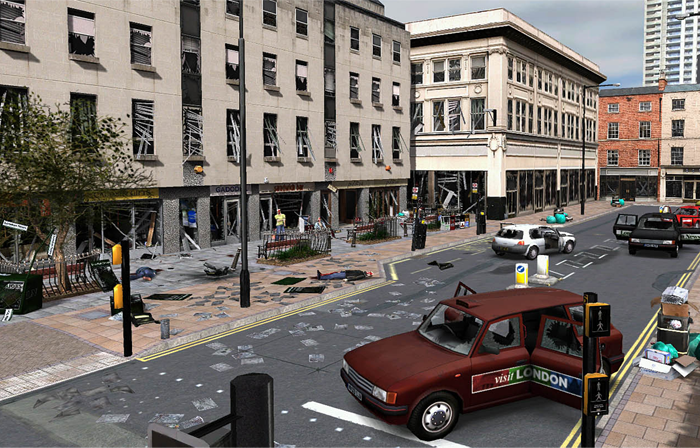
\includegraphics[scale=0.5]{tics/images/triage.png}
\caption{Ambientación de Triage}
\label{fig:triage}
\end{figure}

\emph{Triage Trainer} se desarrolla en una escena de explosión en una calle
(ver~\ref{fig:triage}) la cual es un incidente mayor, y está diseñado para
formar profesionales que puedan participar en una escena de un incidente de este
tipo (médicos, enfermeros, paramédicos, rescatistas). Los jugadores deben
realizar un triage, es decir, evaluar el grado de las lesiones de víctima, las
cuales son generadas aleatoriamente, utilizando los protocolos y controles
médicos adecuados, además de priorizar a las víctimas para el tratamiento. La
apariencia física de cada víctima es imitada con precisión como los signos
vitales, los síntomas y sobre todo los patrones de tiempo para el deterioro de
las lesiones, es decir, la condición de una víctima cambia de forma realista con
el tiempo (ver~\ref{fig:triage_patient1}).

\begin{figure}[h!t]
\centering 
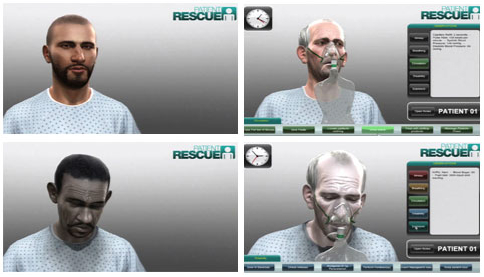
\includegraphics[scale=0.5]{tics/images/patient_side.jpg}
\caption{Evolución de un paciente en Triage}
\label{fig:triage_patient1}
\end{figure}

Al finalizar cada simulación los jugadores reciben retroalimentación acerca de
su rendimiento, incluyendo la precisión de sus chequeos, si los pacientes fueron
priorizados en el orden correcto y el tiempo que les llevó completar el triage,
en comparación con la de un experto.

La retroalimentación de los participantes que utilizaron Triage Trainer sugiere
que el mismo cumplió exitosamente sus fines. Los jugadores asociaron su
experiencia de juego con su experiencia en el mundo real y muchos de ellos
sentían que realmente estaban allí. Se espera que los jugadores puedan tomar
decisiones bajo presión, lo que ayudará a su desarrollo cognitivo. También se
observó que los jugadores tienden a discutir sus experiencias con sus compañeros
de curso, lo que también podría tener un impacto en su aprendizaje.

Un elemento que no fue evaluado por \emph{TruSim} debido a que no era
logísticamente posible fue el impacto de las pruebas en la retención del
conocimiento y el cambio de comportamiento de los
jugadores\cite{education:games}. 


\subsection{Caso 2 SimVenture}

\begin{description}
\item[Tipo:] Juego de simulación de negocios.
\item[Destinatarios:] Personas de 14 a 30 años.
\item[Contenido:] Las realidades de la creación y funcionamiento de un negocio.
\item[Desarrollador:] \emph{Venture Simulations.}
\end{description}

En el inicio del juego (ver~\ref{fig:simventure_tutorial}), a los jugadores se
les brinda informaciones y antecedentes para que que se ubiquen en escena. Ellos
deben empezar a dirigir su propio negocio en su casa de fabricación y venta de
computadoras, mientras deben mantener un trabajo de tiempo completo
independiente. El juego lleva a los jugadores a la ejecución de un negocio en su
propia casa y a la extensión del mismo a más locales, lo que requiere
contratación de personal. Los jugadores son capaces de avanzar en el juego a
través del aprendizaje de los elementos importantes de la empresa, organizadas
en cuatro categorías: organización, ventas/marketing, finanzas y operaciones.
Los jugadores toman decisiones acerca de las actividades dentro de estas áreas y
observan los resultados de sus acciones. 

\begin{figure}[h!]
\centering 
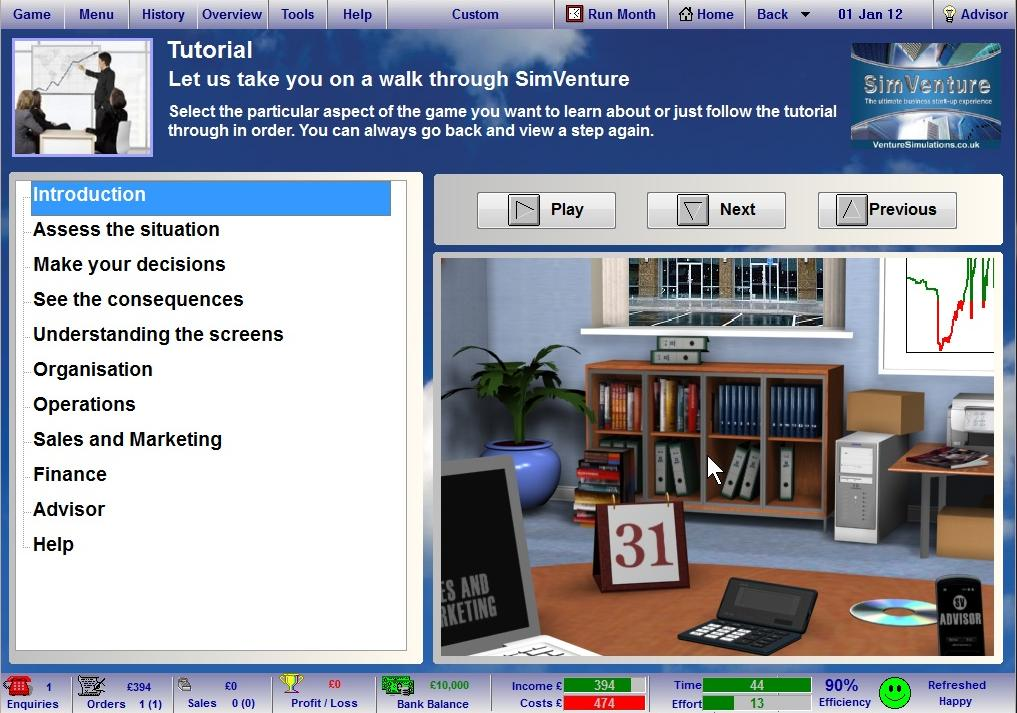
\includegraphics[scale=0.5]{tics/images/simventure-tutorial.jpg}
\caption{Tutorial de SimVenture}
\label{fig:simventure_tutorial}
\end{figure}

Los jugadores obtienen retroalimentación sobre un número de diferentes
parámetros. En un nivel básico, se puede simplemente revisar la cantidad de
ingresos que están generando. Además de esto, el éxito puede ser medido por la
cantidad de pedidos que han recibido para sus productos. También se proporciona
retroalimentación visual para representar la eficiencia de la organización y su
felicidad como individuo.

\emph{Phil Warren}, director de estudios de negocios en \emph{Snaith School}, ha
utilizado \emph{SimVenture} como complemento al plan de estudios. Según el
mismo, el plan de estudios por lo general sólo requiere que los estudiantes
aprendan sobre los diversos elementos del negocio de forma aislada, sin embargo
en la realidad, cualquier decisión que se tome en una de las partes de un
negocio tiene efecto en las demás. \emph{SimVenture} se vio como una oportunidad
de aplicar los conocimientos aprendidos en clase en una actividad práctica,
además se observó que permitir que los estudiantes jueguen en pares da un
espacio para la discusión en torno a las decisiones y aprenden de sus errores
juntos\cite{education:games}.

